\section{Data Preparation}
\begin{frame}
    \sectionpage
\end{frame}

\begin{frame}
    \frametitle{Processing Markers Data}

    \begin{itemize}
        \item Hierarchical clustering by complete distance ...
        \item Select representative markers.
        \item Marginal gene-marker association analysis.
    \end{itemize}
\end{frame}

\begin{frame}
    \frametitle{Processing Expression Level Data}

    We choose genes according to MAPK signaling pathways \footnote[2]{Kanehisa, M., Goto, S., Sato, Y., Kawashima, M., Furumichi, M. and Tanabe, M. (2014) Data, information, knowledge and principle: Back to metabolism in KEGG. Nucleic Acids Res., 42, D199–D205.}

    \begin{figure}[h]
        \centering
        \includegraphics[width=0.75\textwidth]{./figs/MAPK.png}
    \end{figure}
\end{frame}



\section{Methodology}
\begin{frame}
    \sectionpage
\end{frame}

\begin{frame}
    \frametitle{Lasso}

    Let $Y_j$ denote the $j$-th column of $Y$, represent the expression level of $j$-th gene. 

    An intuitive method is to regress each $Y_j$ by $X$, so we can get $q$ linear models. 
    We can use LASSO to estimate the coefficient vector $\beta_{(j)}$. 
    
    And then combind $q$ coefficient vector $\beta_{(j)}$ into a coefficient matrix $\mathbb{\beta}$ by columns. 
\end{frame}

\begin{frame}
    \frametitle{Result of LASSO}

    \begin{figure}[h]
        \centering
        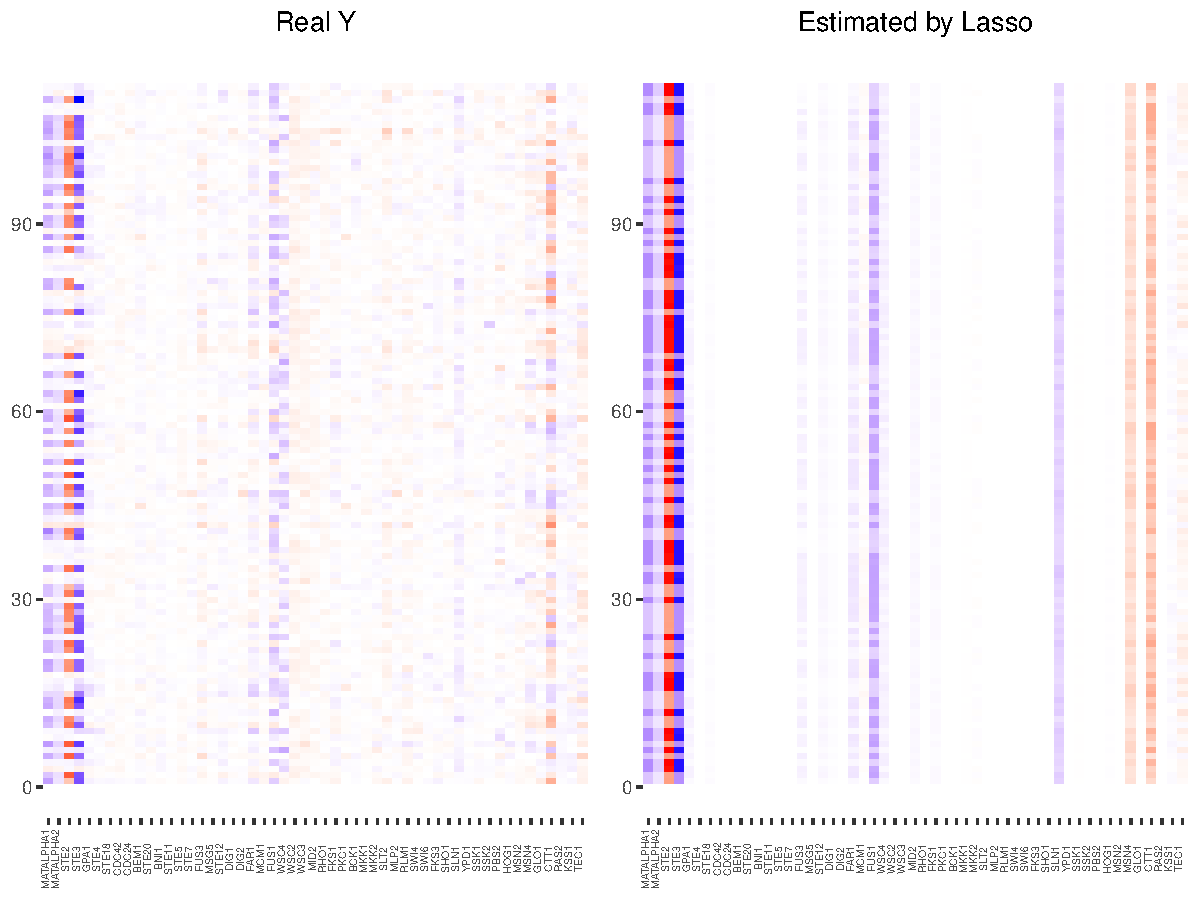
\includegraphics[width=0.8\textwidth]{./figs/lasso.pdf}
        \caption{Heatmaps of real $Y$ and $\hat{Y}$ by LASSO}
    \end{figure}
\end{frame}

\begin{frame}
    \frametitle{Result of LASSO}
    LASSO is a kind of shinkage estiamtion method. 
    An sparse $\beta_{(j)}$ is expected for each $j\in\{ 1,2,\dots,q \}$. 

    But $\mathbb{\beta}$ may not be sparse. 
    Actually, there are $602$ nonzero rows in $\mathbb{\beta}$ which is also of full column rank. 
\end{frame}

\begin{frame}{Multi-response regression}
    Let $X$ denote the eQTLs matrix, $Y$ denote the genes expression matrix, $E$ the random error matrix, and $C$ the coefficient matrix, we construct the multi-response linear model
    \begin{equation*}
        Y = XC + E
    \end{equation*}
    
    We introduce a penalty function to estimate $C$. 
    Firstly, we consider the SVD decomposition $C= UDV$ and then compose penalty into $U$, $D$ and $V$ simultaneously. 
    \begin{equation*}\footnotesize
        \begin{split}
            (\widehat{\mathbf{D}}, \widehat{\mathbf{U}}, \widehat{\mathbf{V}})
            = & \underset{\mathbf{D}, \mathbf{U}, \mathbf{V}}{\arg \min }\left\{\frac{1}{2}\left\|\mathbf{X}-\mathbf{U D V}^{T}\right\|_{F}^{2}+\lambda_{d}\|\mathbf{D}\|_{1}+\lambda_{a} \rho_{a}(\mathbf{U D})+\lambda_{b} \rho_{b}(\mathbf{V D})\right\} \\ 
            & \text { subject to } \mathbf{U}^{T} \mathbf{U}=\mathbf{I}_{m}, \quad \mathbf{V}^{T} \mathbf{V}=\mathbf{I}_{m} 
        \end{split}
    \end{equation*}
\end{frame}

\begin{frame}
    \frametitle{Result of SOFAR}
    \begin{figure}[h]
        \centering
        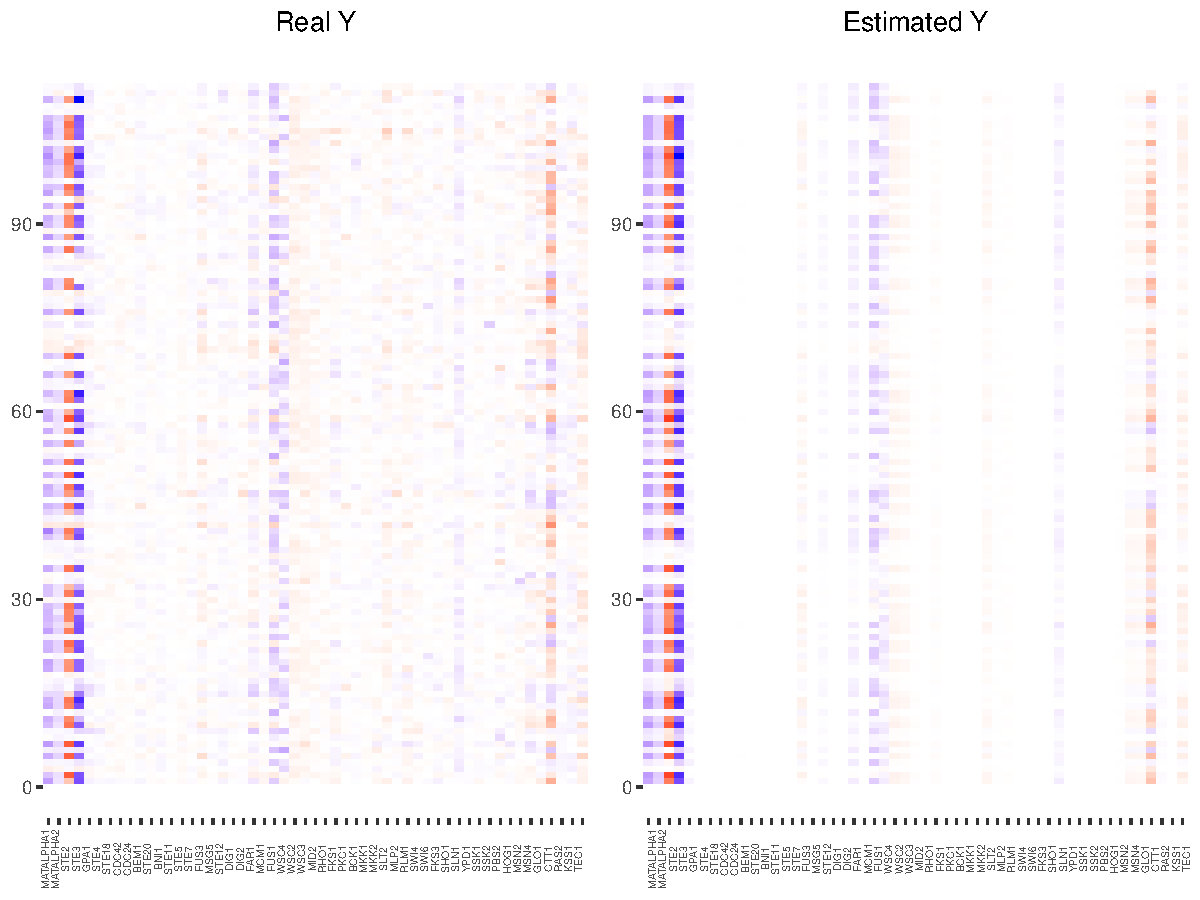
\includegraphics[width=0.8\textwidth]{./figs/heatmap1.pdf}
        \caption{Heatmaps of real $Y$ and $\hat{Y}$ by SOFAR}
    \end{figure}
\end{frame}

\begin{frame}
    \frametitle{Result of SOFAR}
    \begin{figure}[h]
        \centering
        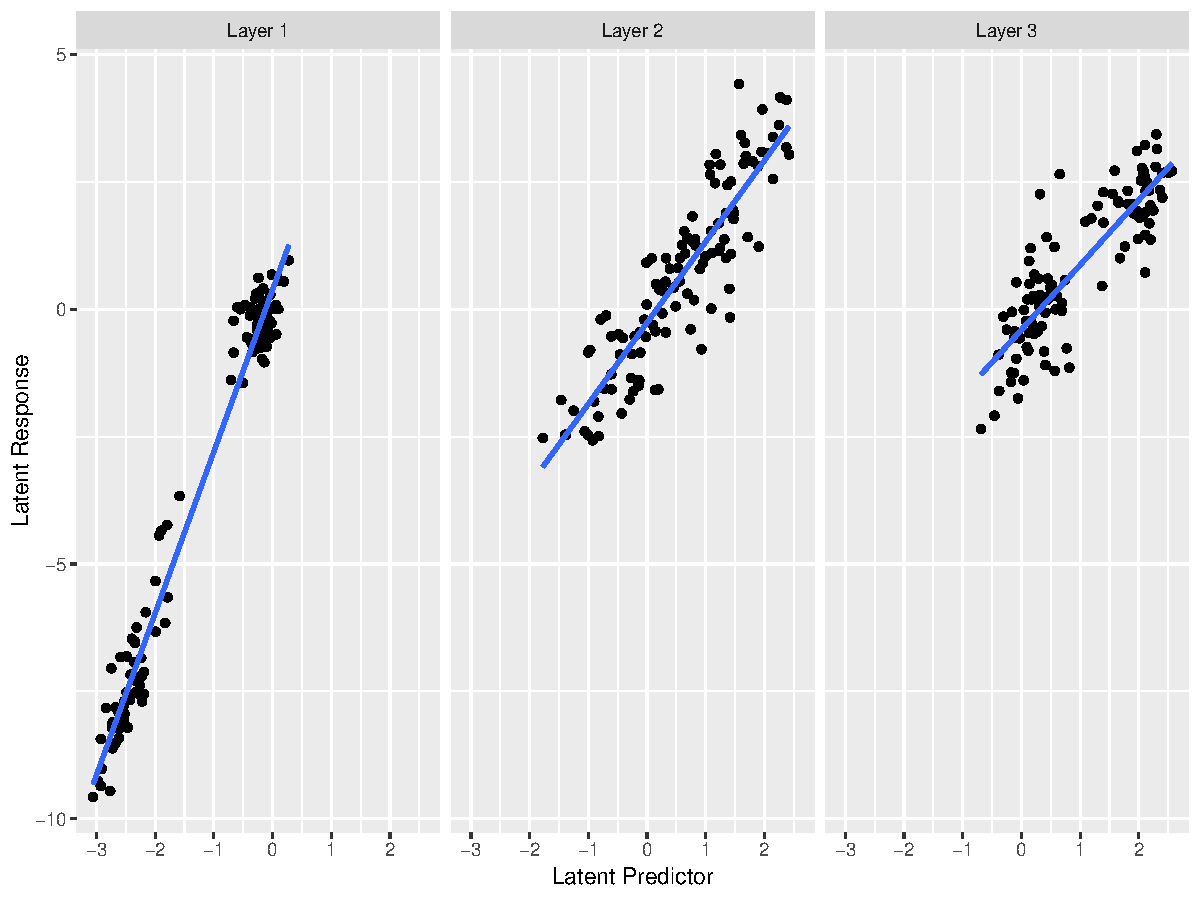
\includegraphics[width=0.75\textwidth]{./figs/latent1.pdf}
        \caption{Scatterplots of the latent responses versus the latent predictors in three SVD layers for the yeast data estimated by the SOFAR method}
    \end{figure}
\end{frame}


\begin{frame}
    \frametitle{Further Reduce Dimension of Markers}

    We performed a marginal gene-marker association analysis to identify markers that are associated with the expression levels of at least two genes with a p-value less than $0.05$, resulting in a total of $p = 776$ markers.

    Reduce $18.2\%$ markers.  

    Result: rank $3$ with $228$ non-zero rows in the estimation of $U$ and $25$ non-zero rows in the estimation of $V$. 
\end{frame}


\begin{frame}
    \frametitle{Result of SOFAR after Reduction}
    \begin{figure}[h]
        \centering
        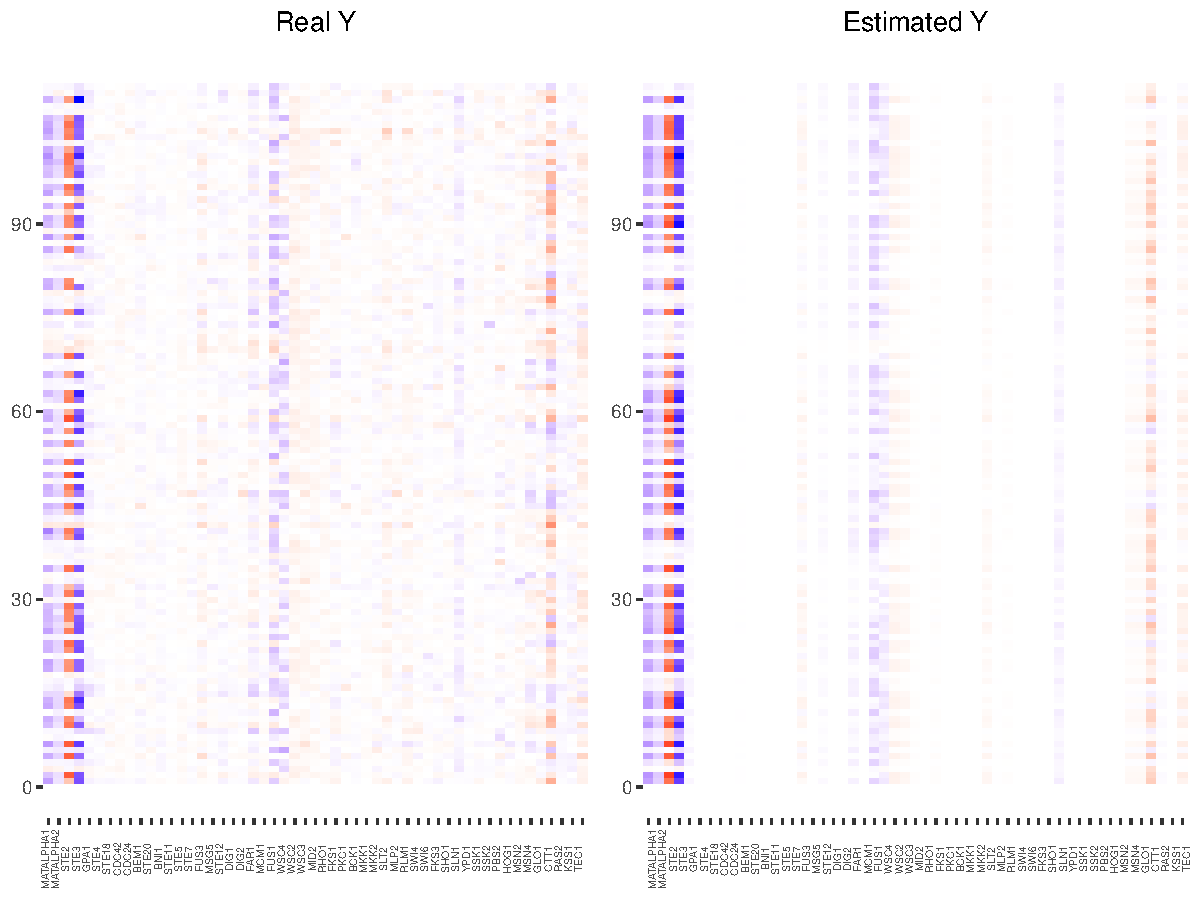
\includegraphics[width=0.8\textwidth]{./figs/heatmap2.pdf}
        \caption{Heatmaps of real $Y$ and $\hat{Y}$ by SOFAR}
    \end{figure}
\end{frame}

\begin{frame}
    \frametitle{Result of SOFAR after Reduction}
    \begin{figure}[h]
        \centering
        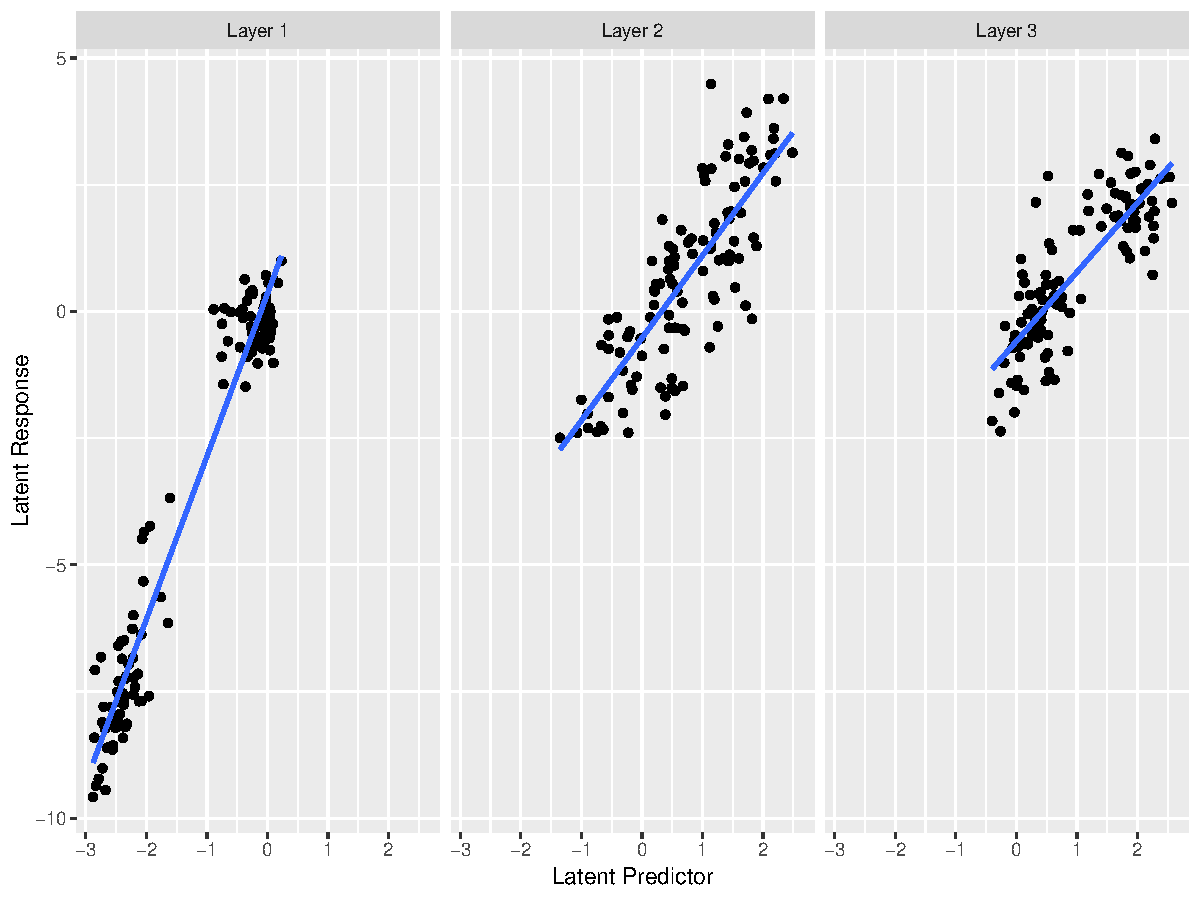
\includegraphics[width=0.75\textwidth]{./figs/letent2.pdf}
        \caption{Scatterplots of the latent responses versus the latent predictors in three SVD layers for the yeast data estimated by the SOFAR method}
    \end{figure}
\end{frame}

\begin{frame} \frametitle{Results of SOFAR}
    \begin{figure}[h]
        \centering
        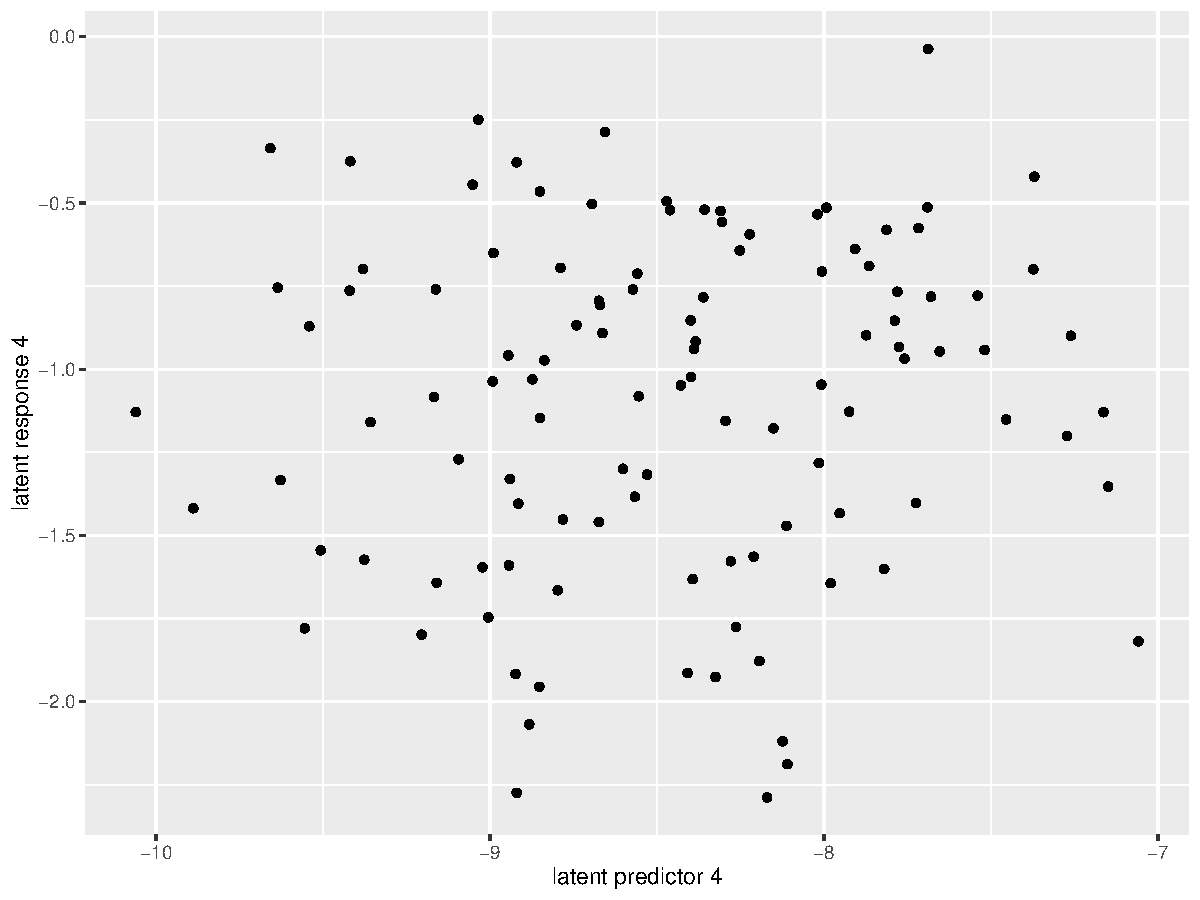
\includegraphics[width=0.75\textwidth]{./figs/latent4.pdf}
        \caption{Scatterplots of the $4$th latent responses versus the latent predictors for the yeast data estimated by the SOFAR method}
    \end{figure}
\end{frame}

